\subsection{The Trusted Platform Module (TPM)}
\label{sec:tpm}

The Trusted Platform Module (TPM) \cite{grawrock2003tpm} introduced the
software attestation model described at the beginning of this section. The TPM
design does not require any hardware modifications to the CPU, and instead
relies on an auxiliary tamper-resistant chip. The TPM chip is only used to
store the attestation key and to perform software attestation. The TPM was
widely deployed on commodity computers, because it does not rely on CPU
modifications. Unfortunately, the cost of this approach is that the TPM has
very weak security guarantees, as explained below.

The TPM design provides one isolation container, covering all the software
running on the computer that has the TPM chip. It follows that the measurement
included in an attestation signature covers the entire OS kernel and all the
kernel modules, such as device drivers. However, commercial computers use a
wide diversity of devices, and their system software is updated at an
ever-increasing pace, so it is impossible to maintain a list of acceptable
measurement hashes corresponding to a piece of trusted software. Due to this
issue, the TPM's software attestation is not used in many security systems,
despite its wide deployment.

The TPM design is technically not vulnerable to any software attacks, because
it trusts all the software on the computer. However, a TPM-based system is
vulnerable to an attacker who has physical access to the machine, as the TPM
chip does not provide any isolation for the software on the computer.
Furthermore, the TPM chip receives the software measurements from the CPU,
so TPM-based systems are vulnerable to attackers who can tap the communication
bus between the CPU and the TPM.

Last, the TPM's design relies on the software running on the CPU to report its
own cryptographic hash. The TPM chip resets the measurements stored in Platform
Configuration Registers (PCRs) when the computer is rebooted. Then, the TPM
expects the software at each boot stage to cryptographically hash the software
at the next stage, and send the hash to the TPM. The TPM updates the PCRs to
incorporate the new hashes it receives, as shown in
Figure~\ref{fig:tpm_measurement}. Most importantly, the PCR value at any point
reflects all the software hashes received by the TPM up to that point. This
makes it impossible for software that has been measured to ``remove'' itself
from the measurement.

\begin{figure}[hbt]
  \centering
  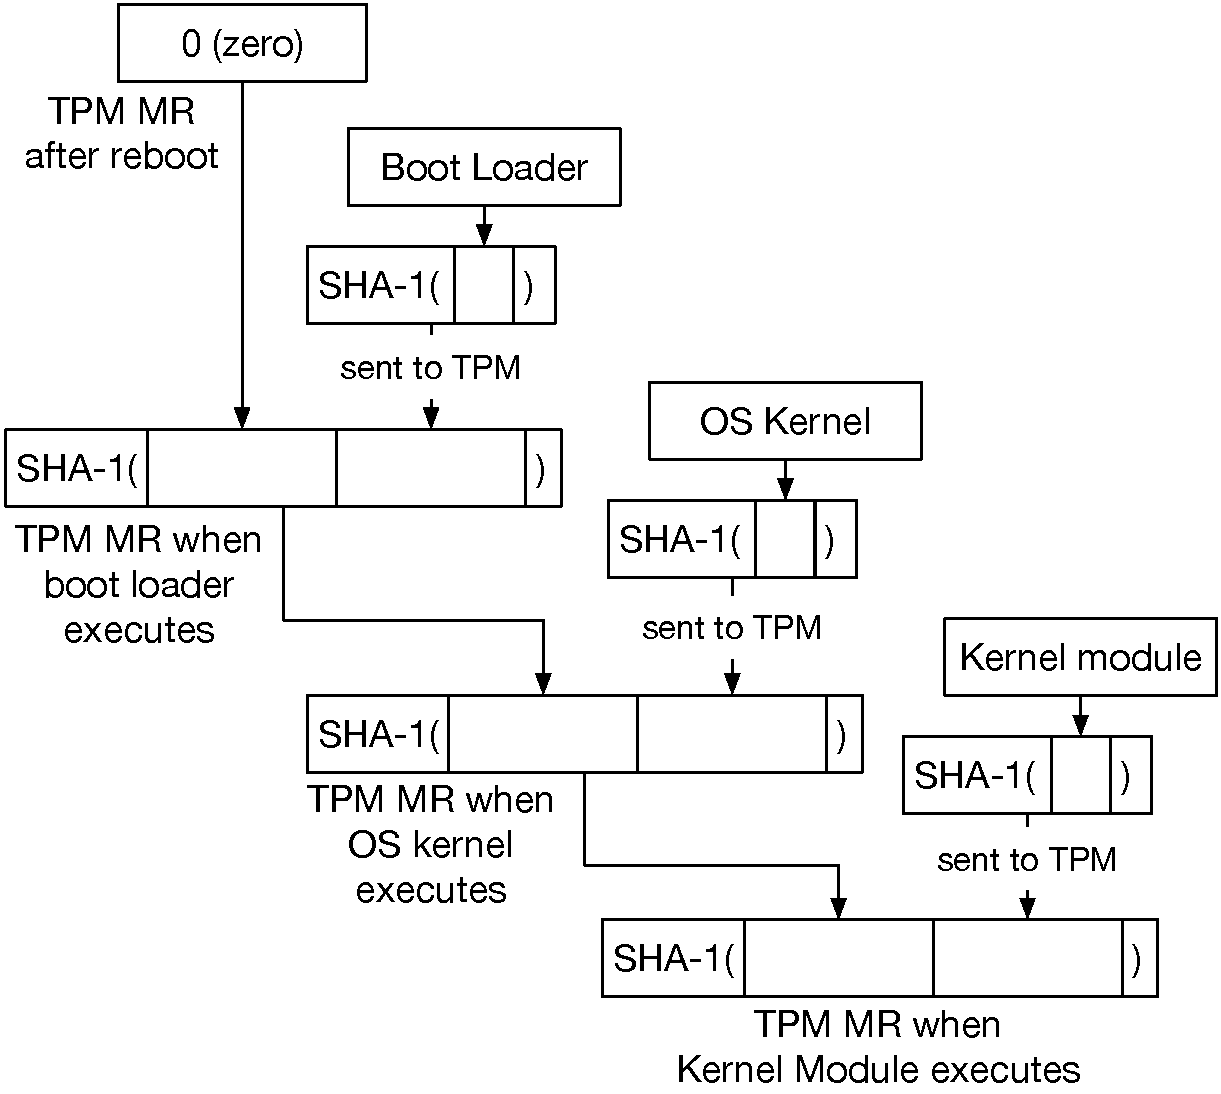
\includegraphics[width=85mm]{figures/tpm_measurement.pdf}
  \caption{
    The measurement stored in a TPM platform configuration register (PCR). The
    PCR is reset when the system reboots. The software at every boot stage
    hashes the next boot stage, and sends the hash to the TPM. The PCR's new
    value incorporates both the old PCR value, and the new software hash.
  }
  \label{fig:tpm_measurement}
\end{figure}

For example, the firmware on most modern computers implement the platform
initialization process in the Unified Extensible Firmware Interface (UEFI)
specification~\cite{forum2015uefi}. Each platform initialization phase is
responsible for verifying or measuring the firmware that implements the next
phase. The SEC firmware initializes the TPM PCR, and then stores the PEI's
measurement into a measurement register. In turn, the PEI implementation
measures the DXE firmware and updates the measurement register that stores the
PEI hash to account for the DXE hash. When the OS is booted, the hash in the
measurement register accounts for all the firmware that was used to boot the
computer.

Unfortunately, the security of the whole measurement scheme hinges on the
requirement that the first hash sent to the TPM must reflect the software that
runs in the first boot stage. The TPM threat model explicitly acknowledges this
issue, and assumes that the firmware responsible for loading the first stage
bootloader is securely embedded in the motherboard. However, virtually every
TPM-enabled computer stores its firmware in a flash memory chip that can be
re-programmed in software (\S~\ref{sec:motherboard}), so the TPM's measurement
can be subverted by an attacker that can reflash the computer's firmware
\cite{butterworth2013bios}.

On very recent Intel processors, the attack described above can be defeated by
having the initialization microcode (\S~\ref{sec:microcode_sec}) hash the
computer's firmware (specifically, the PEI code in UEFI \cite{forum2015uefi}
firwmare) and communicate the hash to the TPM chip. This is marketed as the
Measured Boot feature of Intel's Boot Guard \cite{ruan2014intelme}.

Sadly, most computer manufacturers use Verified Boot (also known as ``secure
boot'') instead of Measured Boot (also known as ``trusted boot''). Verified
Boot means that the processor's microcode only boots into PEI firmware that
contains a signature produced by a key burned into the chip's e-fuses. Verified
Boot does not impact the measurements stored on the TPM, so it does not improve
the security of software attestation.
